% Embedded animations in Beamer
\documentclass{beamer}
% Theme choice
% \usetheme{EastLansing}
\usepackage{sid}
% Required package
\usepackage{animate}
\usepackage{amsmath}
\usepackage{outlines}
\usepackage{bibentry}
\usepackage{chronology}
\nobibliography*
% \usepackage[backend=biber]{biblatex}

\definecolor{links}{HTML}{2A1B81}
\hypersetup{colorlinks,linkcolor=,urlcolor=links}

\usepackage{xr}
\externaldocument{../ch-introduction}
\externaldocument{../ch-literature}
\externaldocument{../ch-simulation}
\externaldocument{../ch-inversion}
\externaldocument{../ch-results}
\externaldocument{../ch-conclusion}
\externaldocument{../ch-appendices}
\graphicspath{{/Users/liamrobinson/Documents/PyLightCurves/docs/build/html/_images}}

\title[]{Light Curve Simulation and Shape Inversion for Human-Made Space Objects}
\author[]{Liam Robinson}
\institute{Purdue Space Information Dynamics Group}
\date{11/13/2023}

% ---------------------------------------------------------------
\begin{document} 
% Configuration
{
    % \usebackgroundtemplate{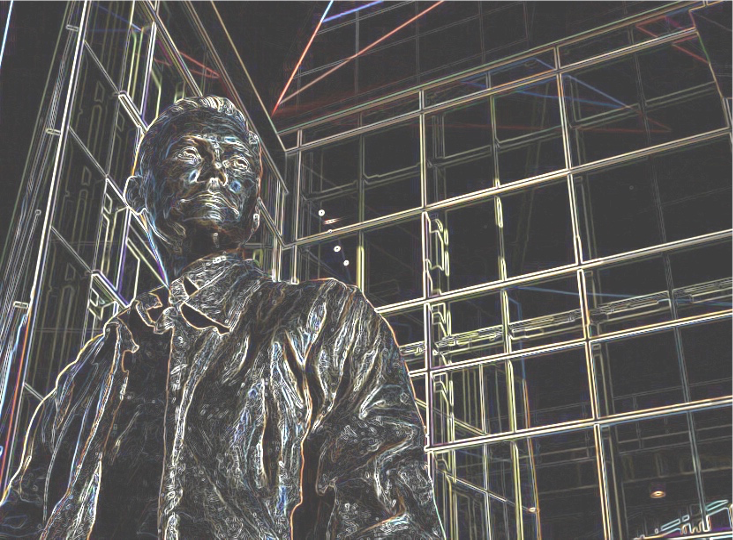
\includegraphics[decodearray={0.3 1.5 0.3 1.5 0.3 1.5},width=\paperwidth,height=\paperheight]{figs_config/neil.png}}
    \usebackgroundtemplate{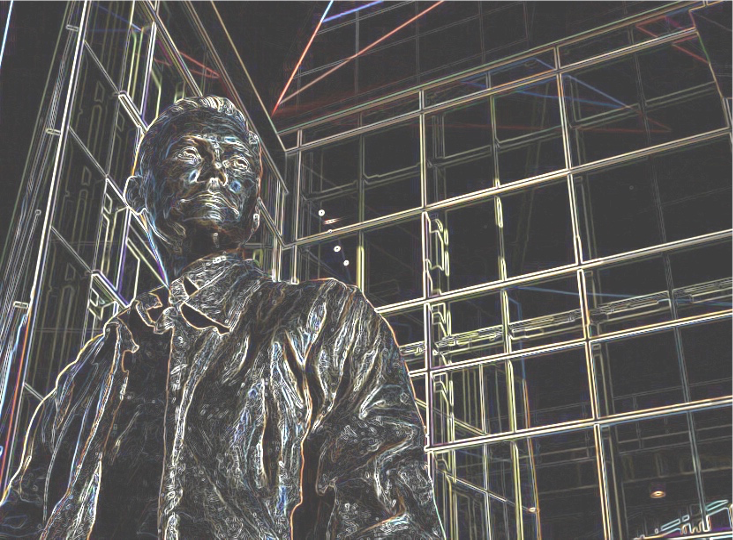
\includegraphics[decodearray={-0.3 0.5 -0.3 0.5 -0.3 0.5},width=\paperwidth,height=\paperheight]{figs_config/neil.png}}
    \begin{frame}[plain]
    \titlepage
    \end{frame}
}
% Set up outline 
\AtBeginSection[]
{
\begin{frame}{Outline}
    \tableofcontents[currentsection]
\end{frame} 
}

\section{Introduction}

\begin{frame}{Motivation}
    \begin{outline}
        \1 Space is becoming more crowded
        \1 We have an imperfect understanding of the space environment
        \1 Understanding the shape of debris objects is important for orbit propagation and active removal
    \end{outline}

    \begin{figure}
        \centering
        \includegraphics[width=0.8\textwidth]{sphx_glr_propagate_catalog_001.png}
        \label{fig:debris}
        \caption{Publicly tracked objects in 2000 and 2023}
    \end{figure}
\end{frame}

\begin{frame}{Research Objectives}
    \begin{outline}
        \1 Developing a high-fidelity light curve simulation framework to simulate the physics of real measurements
        \1 Adapting direct shape inversion techniques for human-made space objects
        \1 Designing a new method for inverting shape with noisy measurements and estimating nonconvex geometry
    \end{outline}
\end{frame}

\begin{frame}{State of The Art: Simulation}

    \begin{outline}
        \1 Light curve simulation literature often assumes:
        \2 Uniform material properties
        \2 Self-shadowing is negligible
        \2 Object geometry is simple \cite{cabrera2021}
        \2 Measurement noise is negligible or Gaussian \cite{fan2020thesis}
    \end{outline}
\end{frame}

\begin{frame}{State of The Art: Shape Inversion}

    \begin{outline}
        \1 Direct shape inversion
        \2 Require \textit{a priori} knowledge of material properties and attitude
        \2 Highest fidelity shape estimates
        \1 Filter-based methods
        \2 Attempt to estimate shape and attitude simultaneously
        \2 Limited to simple geometries
        \1 Deep learning
        \2 Trains models to classify objects by their light curves
        \2 Unpredictable behavior outside the training set
    \end{outline}

    This work presents improvements to direct shape inversion
\end{frame}

\begin{frame}{Direct Inversion Literature Timeline}
    Asteroid Inversion
    \begin{chronology}[4]{2000}{2022}{\textwidth}
        \event{1997}{Russell (1906) \cite{russell1906}}
        \event{2000}{Kaasalainen \cite{kaasalainen2000, kaasalainen2001, kaas2002models}}
        \event{2003}{Durech \cite{durech2003}}
        \event{2014}{Yu \cite{yu2014shape}}
        \event{2022}{Chng \cite{chng2022}}
    \end{chronology}

    Human-made Object Inversion
    \scriptsize{
    \begin{chronology}[4]{2000}{2022}{\textwidth}
        \event{1998}{Ikeuchi (1981) \cite{ikeuchi1981}}
        \event{1999}{Little (1985) \cite{little1985}}
        \event{2003}{Gardner \cite{gardner2003}}
        \event{2007}{Hall \cite{hall2007separating}}
        \event{2014}{Bradley \cite{bradley2014}}
        \event{2019}{Fan \cite{fan2019}}
        \event{2020}{Fan \cite{fan2020thesis} and Friedman \cite{friedman2020}}
        \event{2021}{Cabrera \cite{cabrera2021} and Fan \cite{fan2021}}
        \event{2022}{Robinson \cite{robinson2022} and Friedman \cite{friedman2022}}
    \end{chronology}
    }
\end{frame}

\section{Light Curve Simulation}

\begin{frame}{Light Curve Simulation Outline}
    We must follow the path of photons from the Sun to the observer, answering the following questions along the way:
    \begin{outline}
        \1 How much light does the Sun emit?
        \1 How much light reaches the object?
        \1 How much light is reflected by the object?
        \1 How much light from the object reaches the observer?
        \1 How does the observer collect and measure that light?
    \end{outline}
\end{frame}

\begin{frame}{The Sun}
    \begin{outline}
        \1 The Sun releases different amounts of light as a function of:
        \2 Time within the solar cycle
        \2 Wavelength
        \1 At a given date, the Sun's total irradiance at $1$ AU is $\bar{I}_{s}$
    \end{outline}

    \begin{figure}
        \centering
        \includegraphics[width=0.8\textwidth]{sphx_glr_random_figures_for_defense_pres_001_2_00x.png}
        \label{fig:sun}
        \caption{The Sun's total irradiance and spectrum}
    \end{figure}
\end{frame}

\begin{frame}{Propagation Through Space}
    \begin{outline}
        \1 Accounting for the inverse square law, we find the solar irradiance at the Earth's position with $r_{\mathrm{Sun} \rightarrow \mathrm{Earth}}$ expressed in AU:

        \begin{equation*}
            I_s = \frac{\bar{I}_{s}}{r_{\mathrm{Sun} \rightarrow \mathrm{Earth}}^2}.
        \end{equation*}

    \end{outline}

    \begin{figure}
        \centering
        \includegraphics[width=0.4\textwidth]{sphx_glr_random_figures_for_defense_pres_002_2_00x.png}
        \label{fig:sun}
        \caption{The Sun's total irradiance at the Earth}
    \end{figure}
\end{frame}

\begin{frame}{Orbital Motion --- How does the object move?}
    \begin{outline}
        \1 In unperturbed two-body motion, the relative orbits are conic sections
        \1 Third-body and Earth non-uniform gravity, solar radiation pressure, and atmospheric drag are all important perturbations dependng on the orbital altitude
        \1 The Simplified General Perturbations 4 (SGP4) algorithm approximates some of these perturbations and is used to propagate orbits in this work
        \2 Chosen for availability of Two-Line Elements (TLEs) for publicly-tracked objects 
        \2 Soon to be replaced by SGP4-XP \cite{payne2022}
    \end{outline}
\end{frame}

\begin{frame}{Attitude Motion --- How does the object spin?}
    \begin{outline}
        \1 Environmental torques on space objects do exist on orbit, but can be neglected on the scale of minutes to hours
        \1 Torque-free attitude motion for rigid bodies is described by Euler's equations of motion for an inertia tensor $J$ and body frame angular velocity $\mathbf{\omega}$ \cite{crassidis1ed}:
        \begin{equation*}
            \dot{\mathbf{\omega}} = J^{-1} \left[ \left(J \mathbf{\omega} \right) \times \mathbf{\omega} \right]
        \end{equation*}
        \1 These EOMs are integrated with a quaterion $\mathbf{q} = \left[q_1, q_2, q_3, q_4 \right]^T$ to track the orientation of the body in inertial space \cite{crassidis1ed}:

        \begin{equation*}
            \left[\begin{matrix}\dot{q_1}\\\dot{q_2}\\\dot{q_3}\\\dot{q_4}\\\end{matrix}\right]
            =
            \frac{1}{2}\left[\begin{matrix}q_4&-q_3&q_2&q_1\\q_3&q_4&-q_1&q_2\\-q_2&q_1&q_4&q_3\\-q_1&-q_2&-q_3&q_4\\\end{matrix}\right]
            \left[\begin{matrix}\omega_1\\\omega_2\\\omega_3\\0\\\end{matrix}\right]        
        \end{equation*}
    \end{outline}
\end{frame}

\begin{frame}{Types of Torque-Free Motion}
    \begin{figure}
    \centering
    \begin{subfigure}[b]{0.3\textwidth}
        \centering
        \animategraphics[loop,width=3cm]{30}{imgs/sphx_glr_vis_attitude_motion_001/}{0}{199}
        \label{fig:att1}
        \caption{Spin, precession, and nutation}
    \end{subfigure}
    \hfill
    \begin{subfigure}[b]{0.3\textwidth}
        \centering
        \animategraphics[loop,width=3cm]{30}{imgs/sphx_glr_vis_attitude_motion_002/}{0}{199}
        \label{fig:att2}
        \caption{Spin and precession}
    \end{subfigure}
    \hfill
    \begin{subfigure}[b]{0.3\textwidth}
        \centering
        \animategraphics[loop,width=3cm]{30}{imgs/sphx_glr_vis_attitude_motion_003/}{0}{199}
        \label{fig:att3}
        \caption{Spin only}
    \end{subfigure}
    \hfill
    \end{figure}
\end{frame}

\begin{frame}{Bidirectional Reflectance Distribution Functions (BRDFs)}
    \begin{outline}
        \1 BRDFs describe how light is reflected from a surface
        \2 $f_r(L,O)$ describes the fraction of incident light $L$ reflected in the direction of an observer $O$
        \1 Many formulations exist, but to be relevant to this work, they must \cite{montes2012}:
        \2 Conserve energy for all $L$:
        \[
            \int_{O \in \mathbb{S}^2} f_r(L, O) \: d\mathbb{S}^2 \leq 1
        \]
        \2 Be nonnegative: $f_r(L, O) \geq 0$ for all $L$ and $O$
        \2 Be reciprocal: $f_r(L, O) = f_r(O, L)$ for all $L$ and $O$
        \1 Generally parameterized by:
        \2 Coefficient of diffuse reflectivity $C_d$
        \2 Coefficient of specular reflectivity $C_s$
        \2 Specular exponent $n$ or surface roughness $\alpha$
    \end{outline}
\end{frame}

\begin{frame}{BRDFs in Action}
    \begin{figure}
        \centering
        \includegraphics[width=0.8\textwidth]{sphx_glr_brdf_renders_002_2_00x.png}
        \label{fig:brdfs}
        \caption{BRDFs implemented for this work}
    \end{figure}
\end{frame}

\begin{frame}{Brightness Units}
    \begin{outline}
        \1 Irradiance $I$
        \2 The amount of light energy incident on a surface per unit area per unit time $\left[ \frac{W}{m^2} \right]$
        \1 Apparent magnitude $m$
        \2 Negative logarithm of irradiance relative to a zero point $I_0$
        \begin{equation*}
            m = -2.5 \log_{10}\left( \frac{I}{I_0} \right)
        \end{equation*}
        \1 Normalized irradiance $\hat{I}$
        \2 Irradiance received at a distance $1$ meter from an object illuminated by parallel $1$ $\left[W/m^2\right]$ light rays
        \2 Related to true irradiance by the true distance of the object $r^2$ and the mean irradiance of the Sun $I_s$
        \begin{equation*}
        \hat{I} = \frac{r^2}{I_s} I
        \end{equation*}
    \end{outline}
\end{frame}

\begin{frame}{Time Systems --- What time is it?}
    \begin{outline}
        \1 International Atomic Time (TAI) is based on atomic clocks
        \1 Coordinated Universal Time (UTC) is based on TAI, but has leap seconds added to keep it in sync with Earth's rotation --- which is not constant!
    \end{outline}

    \begin{outline}
        \1 Sidereal time is based on the rotation of the Earth relative to the stars
        \2 Greenwich Mean Sidereal Time (GMST) uses the mean rotation rate of the Earth
        \2 Greenwich Apparent Sidereal Time (GAST) uses the true rotation rate of the Earth
        \1 The Julian Date (JD): the fraction number of days since Wednesday, January 1, 4713 BCE, 12:00 UTC
    \end{outline}
\end{frame}

\begin{frame}{Terrestrial Reference Frames --- Where is the observer?}
    \begin{outline}
        \1 The International Terrestrial Reference Frame (ITRF) is a coordinate frame fixed in the Earth's crust with $\hat{x}$ pointing towards the prime meridian, $\hat{y}$ pointing towards $90^\circ$ east longitude, and $\hat{z}$ pointing towards the north pole
        \1 Given the geodetic latitude $\phi_\mathrm{geod}$, longitude $\lambda$, and altitude $a_{ellip}$ of an observer, the position of the observer in ITRF is given by:
        \begin{align*}
            e^2 &= 2f - f^2 \\
            N &= \frac{R_E}{\sqrt(1 - e^2 \sin(\phi_\mathrm{geod})^2)} \\
            \rho &= (N + a_{ellip}) \cos(\phi_\mathrm{geod}) \\
            x_\mathrm{itrf} &= \rho \cos(\lambda) \\
            y_\mathrm{itrf} &= \rho \sin(\lambda) \\
            z_\mathrm{itrf} &= \left(N (1 - e^2) + a_{ellip} \right) \sin(\phi_\mathrm{geod}). \\          
        \end{align*}
    \end{outline}
\end{frame}

\begin{frame}{Celestial Reference Frames --- Where is the object?}
    \begin{outline}
        \1 J2000 has $\hat{x}$ pointing towards the direction of the vernal equinox on January 1, 2000 12:00 UTC, and $\hat{z}$ normal to the orientation of Earth's equatorial plane on January 1, 2000 12:00 UTC
        \1 Converting from ITRF to J2000 requires accounting for:
        \2 Polar motion, yielding the Greenwich True of Date (GTOD) reference frame
        \2 GMST, yielding the True Equator Mean Equinox (TEME) reference frame
        \2 The difference between GAST and GMST, yielding the True of Date (TOD) reference frame
        \2 Nutation of the Earth's rotation axis since the J2000.0 epoch, yielding the Mean of Date (MOD) reference frame
        \2 Precession of the Earth's rotation axis since the J2000.0 epoch, yielding the J2000 reference frame
        \1 With J2000, all observations at any date can be converted into a common reference frame
    \end{outline}
\end{frame}

\begin{frame}{Observer Constraints --- Can the telescope see the object?}
    To be observable:
    \begin{outline}
        \1 The object must reflect \textit{enough} light
        \1 The observing station must be in eclipse
        \1 The object must be above the horizon
    \end{outline}
\end{frame}

\begin{frame}{Charge Coupled Devices (CCDs)}
    \begin{outline}
        \1 Many telescopes use CCDs to count incoming photons and output a digital signal
        \1 CCDs are composed of a grid of pixels wells, each accumulating a charge in photoelectrons as photons hit them
        \2 The relationship between incident photons and photoelectrons is governed by the quantum efficiency of the CCD
    \end{outline}
\end{frame}

\section{Direct Shape Inversion}

\begin{frame}{The Extended Gaussian Image (EGI)}
\end{frame}

\begin{frame}{EGI Optimization}
\end{frame}

\begin{frame}{EGI Resampling and Merging}
\end{frame}

\begin{frame}{Support Optimization}
    \begin{outline}
        \1 The ``support'' of a face is the perpendicular distance from that face's plane to the origin
        \1 Due to the Minkowski theorem, the support vector of a convex polyhedron is unique
        \1 This support is found by minimizing the mixed volume of the polyhedron:
        \begin{align*}
            & \min_{\vec{h}}\left\{ \vec{h} \cdot \| \vec{E} \| \right\} \\
            & \textrm{such that } \frac{1}{3}\left(\vec{h} \cdot \vec{a} \right) = 1          
        \end{align*}
        \1 Where $\vec{E}$ is the EGI and $\vec{a}$ are the face areas resulting from choosing the support $\vec{h}$
    \end{outline}
\end{frame}

\section{Discussion}

\section{Conclusion}

\begin{frame}{Questions}

\begin{center}
    \animategraphics[loop,width=8cm]{30}{imgs/sphx_glr_plot_earth_001/}{0}{99}
\end{center}
\end{frame}

\bibliographystyle{unsrt}
\bibliography{{/Users/liamrobinson/Documents/PyLightCurves/docs/source/_static/refs.bib}}

\end{document}
